%% 
%% Copyright 2007-2024 Elsevier Ltd
%% 
%% This file is part of the 'Elsarticle Bundle'.
%% ---------------------------------------------
%% 
%% It may be distributed under the conditions of the LaTeX Project Public
%% License, either version 1.3 of this license or (at your option) any
%% later version.  The latest version of this license is in
%%    http://www.latex-project.org/lppl.txt
%% and version 1.3 or later is part of all distributions of LaTeX
%% version 1999/12/01 or later.
%% 
%% The list of all files belonging to the 'Elsarticle Bundle' is
%% given in the file `manifest.txt'.
%% 
%% Template article for Elsevier's document class `elsarticle'
%% with harvard style bibliographic references

\documentclass[preprint,12pt,authoryear]{elsarticle}

%% Use the option review to obtain double line spacing
%% \documentclass[authoryear,preprint,review,12pt]{elsarticle}

%% Use the options 1p,twocolumn; 3p; 3p,twocolumn; 5p; or 5p,twocolumn
%% for a journal layout:
%% \documentclass[final,1p,times,authoryear]{elsarticle}
%% \documentclass[final,1p,times,twocolumn,authoryear]{elsarticle}
%% \documentclass[final,3p,times,authoryear]{elsarticle}
%% \documentclass[final,3p,times,twocolumn,authoryear]{elsarticle}
%% \documentclass[final,5p,times,authoryear]{elsarticle}
%% \documentclass[final,5p,times,twocolumn,authoryear]{elsarticle}

%% For including figures, graphicx.sty has been loaded in
%% elsarticle.cls. If you prefer to use the old commands
%% please give \usepackage{epsfig}

%% The amssymb package provides various useful mathematical symbols
% \usepackage{amssymb}
%% The amsmath package provides various useful equation environments.
% \usepackage{amsmath}
\usepackage{amsmath,amsthm,amssymb,scrextend,mathtools}
\usepackage{hyperref}
\usepackage{newtxmath} %for making indicator function
\usepackage{booktabs}
% \RequirePackage[colorlinks,citecolor=blue,urlcolor=blue,backref=page,backref=page]{hyperref}
%% The amsthm package provides extended theorem environments
%% \usepackage{amsthm}

%% The lineno packages adds line numbers. Start line numbering with
%% \begin{linenumbers}, end it with \end{linenumbers}. Or switch it on
%% for the whole article with \linenumbers.
%% \usepackage{lineno}

\newtheorem{theorem}{Theorem}
\newtheorem{lemma}{Lemma}
\newtheorem{definition}{Definition}
\usepackage{natbib}
\usepackage{adjustbox}
\usepackage{multirow}

\journal{Computational Statistics and Data Analysis}

\begin{document}

% \begin{frontmatter}

%% Title, authors and addresses

%% use the tnoteref command within \title for footnotes;
%% use the tnotetext command for theassociated footnote;
%% use the fnref command within \author or \affiliation for footnotes;
%% use the fntext command for theassociated footnote;
%% use the corref command within \author for corresponding author footnotes;
%% use the cortext command for theassociated footnote;
%% use the ead command for the email address,
%% and the form \ead[url] for the home page:
%% \title{Title\tnoteref{label1}}
%% \tnotetext[label1]{}
%% \author{Name\corref{cor1}\fnref{label2}}
%% \ead{email address}
%% \ead[url]{home page}
%% \fntext[label2]{}
%% \cortext[cor1]{}
%% \affiliation{organization={},
%%            addressline={}, 
%%            city={},
%%            postcode={}, 
%%            state={},
%%            country={}}
%% \fntext[label3]{}

\title{Supplementary Material} %% Article title

%% use optional labels to link authors explicitly to addresses:
%% \author[label1,label2]{}
%% \affiliation[label1]{organization={},
%%             addressline={},
%%             city={},
%%             postcode={},
%%             state={},
%%             country={}}
%%
%% \affiliation[label2]{organization={},
%%             addressline={},
%%             city={},
%%             postcode={},
%%             state={},
%%             country={}}

% \author[label1]{Spencer Wadsworth} %% Author name
% \author[label1]{Jarad Niemi}

%% Author affiliation
% \affiliation[label1]{organization={Iowa State Univerity, Department of Statistics},%Department and Organization
%             addressline={2438 Osborn Dr}, 
%             city={Ames},
%             postcode={50011}, 
%             state={Iowa},
%             country={USA}}

%%Graphical abstract
% \begin{graphicalabstract}
%\includegraphics{grabs}
% \end{graphicalabstract}

%%Research highlights
% \begin{highlights}
% \item Research highlight 1
% \item Research highlight 2
% \end{highlights}
% 
%% Keywords

% 
% \end{frontmatter}

%% Add \usepackage{lineno} before \begin{document} and uncomment 
%% following line to enable line numbers
%% \linenumbers

%% main text
%%

\Huge
\begin{center}
  Supplementary Material
\end{center}
\normalsize





Here we include a simulation study similar to the first study in section (??).
% \ref{sec:simulation_analyses}. 
However, instead of simulating data from a normal distribution, data is 
simulated 
from an exponential distribution with parameter $\lambda = 4$. The same prior 
distribution for $\lambda$ was used in fitting QGP, ORD, and IND models, and the 
same prior distribution was assigned to $n$ in QGP and ORD models and 
$1/\sigma_{\rho}$. The prior for $\lambda$ was 
$\pi(\lambda) \sim N(0, 7^2)\vmathbb{1}\{\lambda > 0\}$, the prior for $n$ was
$\pi(n) \sim N(0, 3000^2)\vmathbb{1}\{n > 0\}$, and the prior for
$1/\sigma_{\rho}$ was
$\pi(1/\sigma_{\rho}) \sim N(0, 3000^2)\vmathbb{1}\{1/\sigma_{\rho} > 0\}$.

Figure \ref{fig:exp_par_fit} shows examples of posterior sample density plots 
for $\lambda$ and $n$. QGP and ORD show similar distributions which tend to be 
a bit wider than the posterior distributions from the IND model. The left side 
of figure \ref{fig:exp_cov_dists} shows the percent coverage of the 500 
simulation replicates for $\lambda$ and $n$. Here, the IND model coverage is 
much closer to the nominal level than in the normal distribution case of the 
previous section. The right side of figure \ref{fig:exp_cov_dists} shows the 
average UWD1, TV, and KLD distances for the five QM methods. Again the 
parametric models tend to perform better than the non-parametric SPL and KDE 
methods with the SPL and KDE performing better as $n$ and $K$ increase.





\begin{figure}

\centering
% \begin{subfigure}
  \centering
  \hspace{-.8cm}
  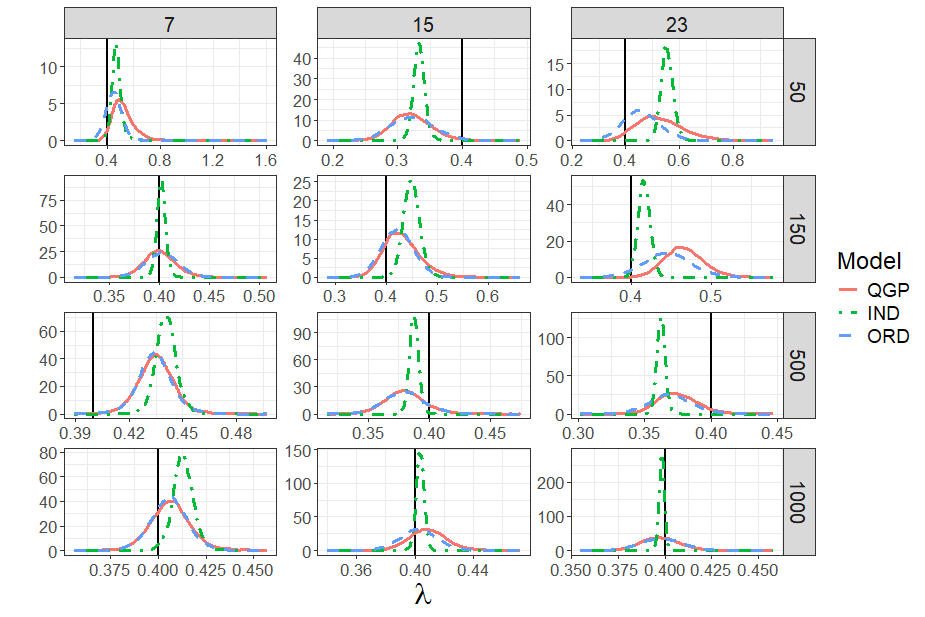
\includegraphics[width=.94\linewidth]{Images/exponential_par_fit.png}
  % \caption{A subfigure}
  % \label{fig:sub1}
% \end{subfigure}%
% \begin{subfigure}
  \centering
  \hspace{-.9cm}
  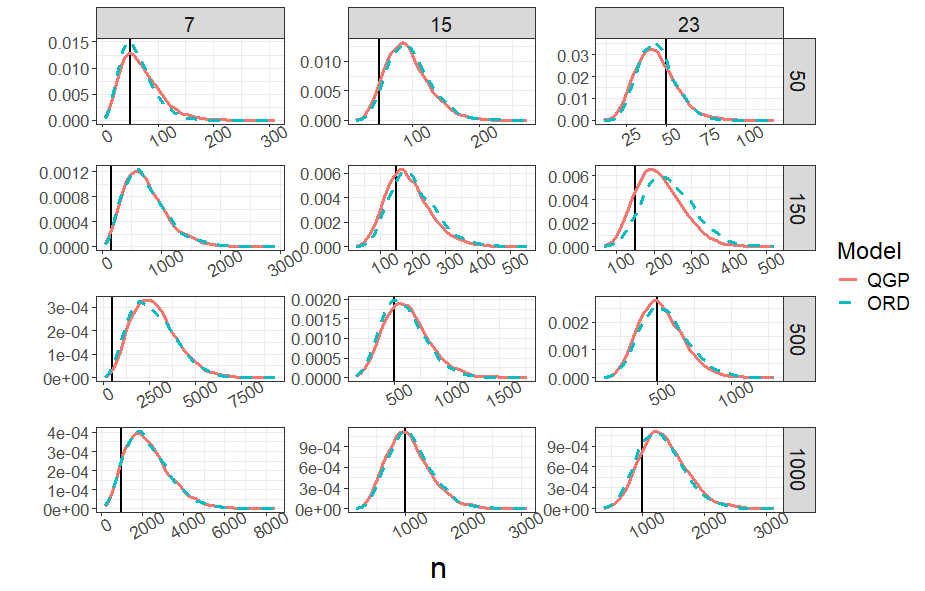
\includegraphics[width=1.05\linewidth]{Images/exponential_n_fit.png}
  % \caption{A subfigure}
  % \label{fig:sub2}
% \end{subfigure}
\caption{Density plots of posterior distribution samples for the exponential 
parameters by QM for QGP, ORD, and IND models. QM was done on estimated 
quantiles from a exponential distribution with parameter $\lambda = 4$. The 
posterior densities are for $\lambda$ (left) and sample size $n$ (right). Plots 
are faceted by true sample size $n \in \{50, 150, 500, 1{,}000\}$ ($y$-axis) 
and number of quantiles $K \in \{7, 15, 23\}$ ($x$-axis). Vertical lines 
(black) show the value of the true parameter.}
\label{fig:exp_par_fit}
\end{figure}





\begin{figure}[hbt!]
% \begin{subfigure}
  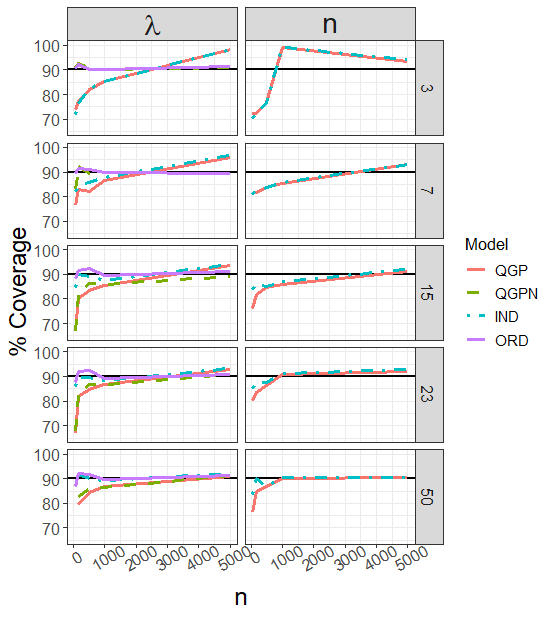
\includegraphics[width=\linewidth]{Images/exponential_coverage.png}
  % \caption{}
  % \label{MLEDdet}
% \end{subfigure}\hfill % <-- "\hfill"
% \begin{subfigure}
  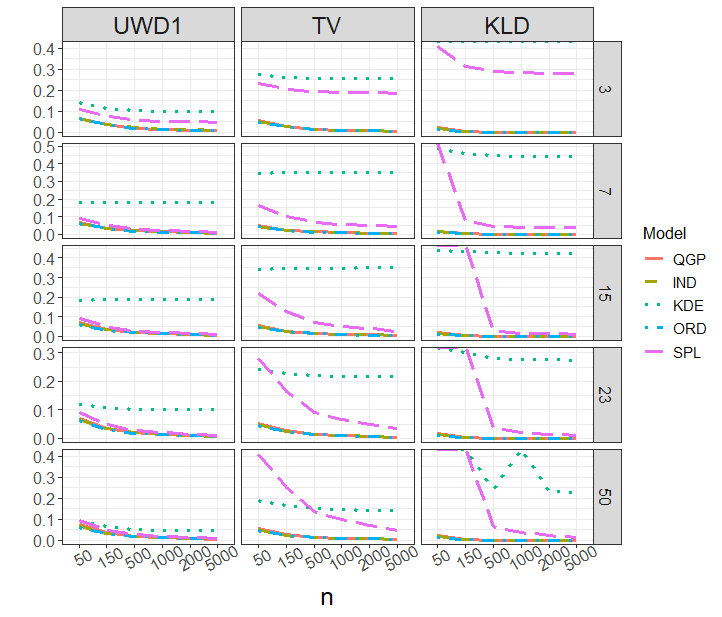
\includegraphics[width=\linewidth]{Images/exponential_dists.png}
  % \caption{}
  % \label{energydetPSK}
% \end{subfigure}
\caption{Posterior coverage (left) calculated as the percentage of times the 
true parameter fell within the modeled 90\% credible interval over the 500 
replications. Coverage is faceted by the exponential parameter 
$\lambda$ and $n$ with $K \in \{3, 7, 15, 23, 50\}$, and by increasing sample 
size ($x$-axis). The five models QGP, ORD, QGPN, ORDN, and IND are colored as 
shown the legend. The horizontal line (black) is at the nominal 90\% level. 
Only QGP and ORD appear for the parameter $n$ as they are the only two which 
estimate an unknown $n$.
Distance between the true distribution and the estimated QM predictive 
distribution (right) averaged over the 500 replications. Distances include 
UWD1, TV, and KLD for $K \in \{3, 7, 15, 23, 50\}$, and by increasing sample 
size ($x$-axis).}
\label{fig:exp_cov_dists}
\end{figure}









\begin{figure}[hbt!]
\centering
%\begin{subfigure}{.5\textwidth}
  \centering
  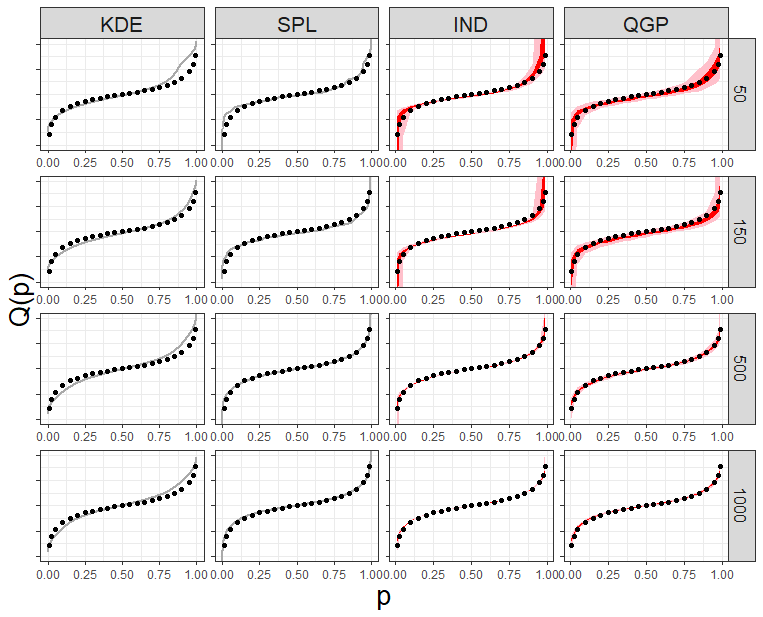
\includegraphics[width=.49\linewidth]{Images/quants_lp.png}
  % \caption{A subfigure}
  % \label{fig:sub1}
%\end{subfigure}%
%\begin{subfigure}{.5\textwidth}
  \centering
  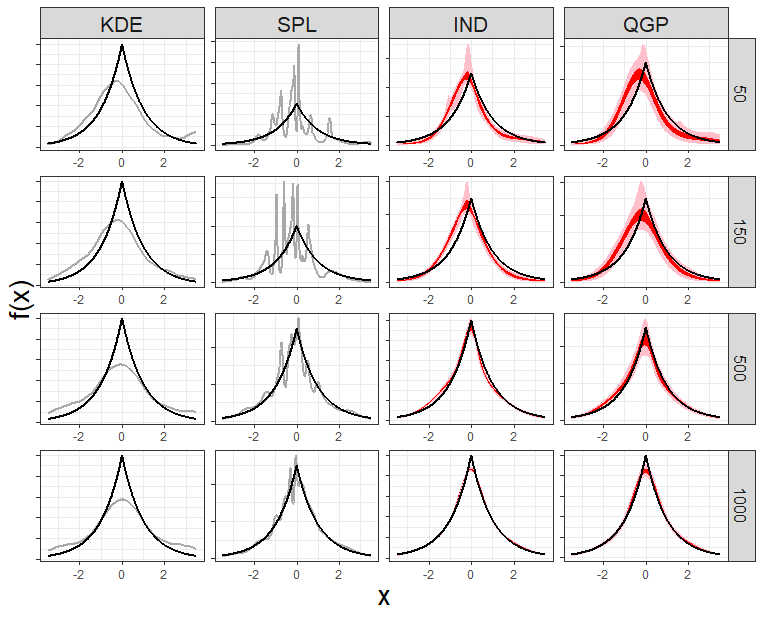
\includegraphics[width=.49\linewidth]{Images/dens_lp.png}
  % \caption{A subfigure}
  % \label{fig:sub2}
%\end{subfigure}
\caption{QM fits of $K=23$ quantiles by KDE, SPL, IND, and QGP for $n \in \{50, 150, 500, 1{,}000\}$. The quantiles were sampled from the Laplace distribution $La(0,1)$. The quantile fits (left) show the true quantiles (black) with either the QM fit line (grey) or the credible intervals of 50\% (red) and 95\% (pink). 
The estimated PDF plots (right) show the true PDF (black) with either a the QM estimated PDF (grey) or the credible intervals of 50\% (red) and 95\% (pink).}
\label{fig:lp_fits}
\end{figure}


\begin{figure}[hbt!]
\centering
%\begin{subfigure}{.5\textwidth}
  \centering
  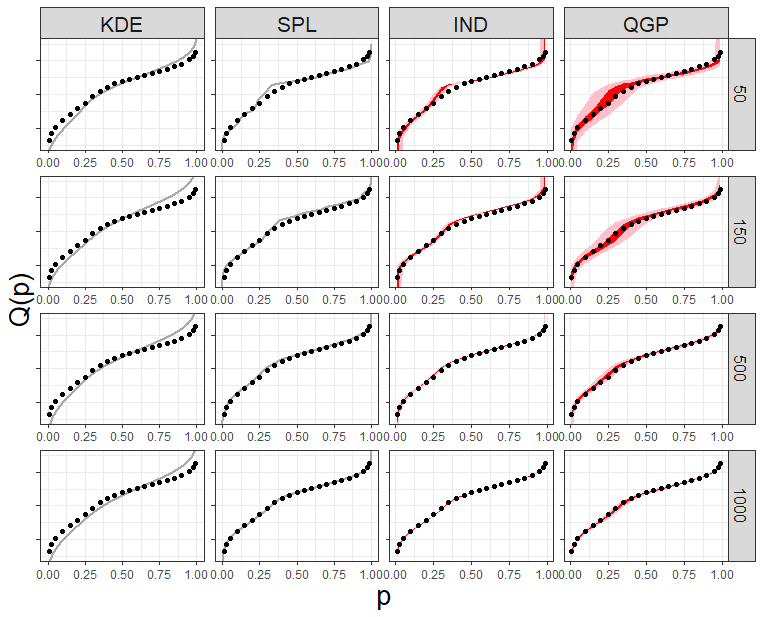
\includegraphics[width=.49\linewidth]{Images/quants_gmix.png}
  % \caption{A subfigure}
  % \label{fig:sub1}
%\end{subfigure}%
%\begin{subfigure}{.5\textwidth}
  \centering
  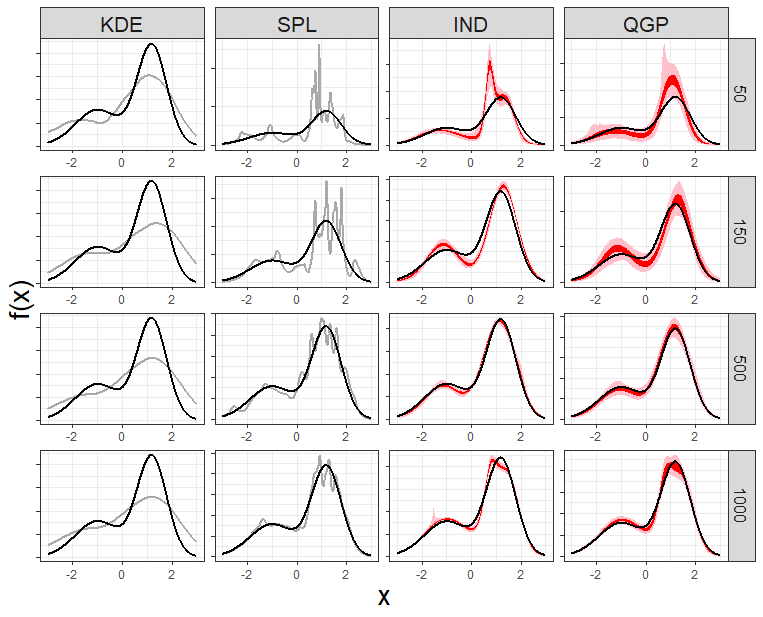
\includegraphics[width=.49\linewidth]{Images/dens_gmix.png}
  % \caption{A subfigure}
  % \label{fig:sub2}
%\end{subfigure}
\caption{QM fits of $K=23$ quantiles by KDE, SPL, IND, and QGP for $n \in \{50, 150, 500, 1{,}000\}$. The quantiles were sampled from the two component normal mixture distribution $w N(-1, 0.9) + (1-w)N(1.2, .6)$ where $w = 0.35$. The quantile fits (left) show the true quantiles (black) with either the QM fit line (grey) or the credible intervals of 50\% (red) and 95\% (pink). 
The estimated PDF plots (right) show the true PDF (black) with either a the QM estimated PDF (grey) or the credible intervals of 50\% (red) and 95\% (pink). }
\label{fig:gmix_fits}
\end{figure}


\begin{figure}[hbt!]
\centering
  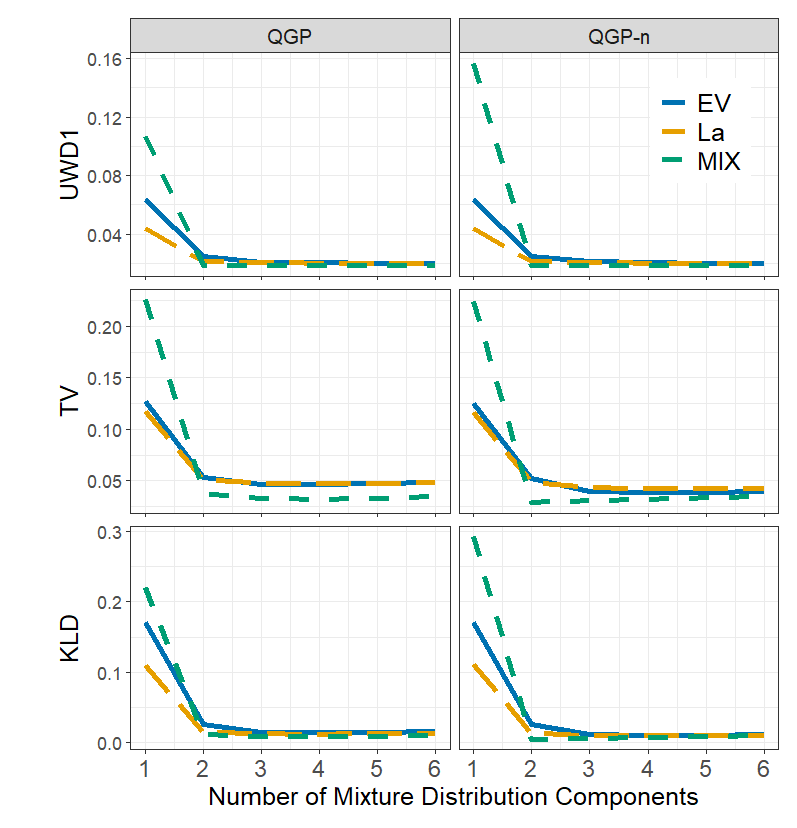
\includegraphics[]{Images/mix_comps.png}
\caption{Future caption}
\label{fig:mix_comps}
\end{figure}


% \begin{table}[hbt!]
% \footnotesize
% \centering
% \caption{UWD1}
% \begin{adjustbox}{center}
% \begin{tabular}{lcccccc|cccccc}
%  & \multicolumn{6}{c}{QGP} & \multicolumn{6}{c}{QGP-n} \\
% \cmidrule(lr){2-7} \cmidrule(lr){8-13}
% Components & 1 & 2 & 3 & 4 & 5 & 6 & 1 & 2 & 3 & 4 & 5 & 6 \\
% \midrule
% EV & 0.063 & 0.025 & 0.021 & 0.020 & 0.020 & 0.020 & 
%       0.064 & 0.025 & 0.021 & 0.021 & 0.020 & 0.020\\
% La & 0.044 & 0.022 & 0.020 & 0.020 & 0.020 & 0.020 & 
%       0.044 & 0.021 & 0.020 & 0.020 & 0.020 & 0.020 \\
% MIX & 0.107 & 0.018 & 0.019 & 0.019 & 0.019 & 0.019 & 
%       0.157 & 0.018 & 0.019 & 0.018 & 0.018 & 0.018
% \end{tabular}
% \end{adjustbox}
% \end{table}












\begin{table}[hbt!]
\footnotesize
\centering
\caption{UWD1}
\begin{adjustbox}{center}
\begin{tabular}{clcccccc|cccccc}
& & \multicolumn{6}{c}{QGP} & \multicolumn{6}{c}{QGP-n} \\
\cmidrule(lr){3-8} \cmidrule(lr){9-14}
& Components & 1 & 2 & 3 & 4 & 5 & 6 & 1 & 2 & 3 & 4 & 5 & 6 \\
\midrule
\multirow{3}{*}{UWD1} &
EV & 0.063 & 0.025 & 0.021 & 0.020 & 0.020 & 0.020 & 
      0.064 & 0.025 & 0.021 & 0.021 & 0.020 & 0.020\\
 & La & 0.044 & 0.022 & 0.020 & 0.020 & 0.020 & 0.020 & 
      0.044 & 0.021 & 0.020 & 0.020 & 0.020 & 0.020 \\
 & MIX & 0.107 & 0.018 & 0.019 & 0.019 & 0.019 & 0.019 & 
      0.157 & 0.018 & 0.019 & 0.018 & 0.018 & 0.018 \\
      \hline
\multirow{3}{*}{TV} &
EV & 0.127 & 0.053 & 0.047 & 0.047 & 0.048 & 0.049 &
      0.125 & 0.052 & 0.039 & 0.039 & 0.039 & 0.039\\
 & La & 0.117 & 0.051 & 0.047 & 0.047 & 0.048 & 0.048 &
      0.117 & 0.048 & 0.043 & 0.043 & 0.043 & 0.042 \\
 & MIX & 0.226 & 0.038 & 0.033 & 0.032 & 0.033 & 0.034 &
      0.225 & 0.029 & 0.031 & 0.032 & 0.034 & 0.035 \\
      \hline
\multirow{3}{*}{KLD} &
EV & 0.171 & 0.025 & 0.014 & 0.013 & 0.014 & 0.015 & 
      0.170 & 0.025 & 0.011 & 0.010 & 0.010 & 0.010\\
& La & 0.110 & 0.014 & 0.012 & 0.012 & 0.012 & 0.012 & 
      0.111 & 0.013 & 0.010 & 0.010 & 0.010 & 0.010 \\
& MIX & 0.221 & 0.010 & 0.008 & 0.008 & 0.009 & 0.010 & 
      0.293 & 0.004 & 0.006 & 0.007 & 0.009 & 0.010
\end{tabular}
\end{adjustbox}
\end{table}






\end{document}


%% For citations use: 
%%       \citet{<label>} ==> Lamport (1994)
%%       \citep{<label>} ==> (Lamport, 1994)
%%
% Example citation, See \citet{lamport94}.

%% If you have bib database file and want bibtex to generate the
%% bibitems, please use
%%
\bibliographystyle{elsarticle-harv}
\bibliography{master_bib}

%% else use the following coding to input the bibitems directly in the
%% TeX file.

%% Refer following link for more details about bibliography and citations.
%% https://en.wikibooks.org/wiki/LaTeX/Bibliography_Management

% \begin{thebibliography}{00}
% 
% %% For authoryear reference style
% %% \bibitem[Author(year)]{label}
% %% Text of bibliographic item
% 
% \bibitem[Lamport(1994)]{lamport94}
%   Leslie Lamport,
%   \textit{\LaTeX: a document preparation system},
%   Addison Wesley, Massachusetts,
%   2nd edition,
%   1994.
% 
% \end{thebibliography}



\endinput
%%
%% End of file `elsarticle-template-harv.tex'.


